\newpage
\section{Modeling User Content Generation}
In this section, we first describe the desired properties of our user content generation model, and briefly discuss some unsuccessful model attempts. We then introduce our factor based user content generation model for CQA platforms.

\subsection{Desiderata} 
To better understand the dynamics of user content generation in CQA platforms, we opt for a model with the following desired properties.

D1. \textit{Macro-scale:} The model should capture user content generation in CQA at aggregate level. 

D2. \textit{Explanatory:} The model should give us some deeper understanding of how the aggregate user community generates content.

D3. \textit{Predictive:} The model should allow us to make predictions about future content generation and relevant aspects.

D4. \textit{Minimalistic:} The model should have as few parameters as necessary, and still closely reflect reality.

D5. \textit{Comprehensive:} The model should encompass the dynamics of content generation for different types of content (e.g., question, answer, comment) in varieties of CQA platforms.

\subsection{Some Unsuccessful Attempts} 
We considered several alternative models to comprehend the content generation dynamics in CQA platforms. Our first attempt was to model user content generation as \lq self-exciting\rq\ point process. In this attempt, we designed and implemented several variants of Hawkes process. Our second attempt was to model user content generation using \lq stage-structured\rq\ projection matrix. In this attempt, we built variants of Leftkovitch matrix. Although both variants of models showed promise, they failed to meet one or more requirements mentioned above. In particular, the Hawkes process based models lacked long term prediction accuracy, while the Leftkovitch matrix based models lacked prediction accuracy and minimalism (large number of parameters). 

\subsection{Factor Based Model} 
Motivated by the macroeconomic production models, we focused on designing factor based model for user content generation in CQA platforms. Instead of directly modeling user content generation as a dynamic process (function of time), we model it in terms of associated factors, which themselves are dynamic. From this point forward, we report the factors of content generation for different content types, discuss basis functions to capture the effect of a single factor and aggregate functions to capture the interaction among multiple factors, and introduce alternative models based on the basis and aggregate functions.

\textbf{Factors of Content Generation.} We recognize two key factors that drive content generation in CQA platforms, namely user participation and content dependency.

\uline{User Participation:} The number of active users is the most important factor in deciding the number of generated content. The participation of more users induce more questions, answers, and comments in a CQA platform.

\begin{table}[thb]
	\centering
	\begin{tabular}{cl}
	\hline
	\textbf{Symbol} & \textbf{Definition}\\ \hline
	$U_q(t)$ & \# of users who asked questions at time $t$\\ 
	$U_a(t)$ & \# of users who answered questions at time $t$\\
	$U_c(t)$ & \# of users who made comments at time $t$\\
	$N_q(t)$ & \# of active questions at time $t$\\
	$N_a(t)$ & \# of answers to active questions at time $t$\\
	$N_c^q(t)$ & \# of comments to active questions at time $t$\\
	$N_c^a(t)$ & \# of comments to active answers at time $t$\\
    $N_c(t)$ & \# of comments to active questions/answers at time $t$\\
	$f_w$ & The functional relationship for content $w$\\ \hline
	 \end{tabular}
    \caption{Notations used in the models}
    \label{tab:notations}
\end{table}

\uline{Content Dependency:} While user participation is vital for content generation, content dependency also affects the number of generated content for different types. Content dependency implies the dependency of a type of content on other type of content(s). For example, answer generation relies on question generation-- in absence of questions, there will be no answers. %Similarly, comment generation relies on both question and answer generation.

In the light of the above discussion, we identify the key factors of content generation in Stack Exchange websites for three primary content types: question, answer, and comment. Figure~\ref{fig:content_factors} shows these factors using notations from Table~\ref{tab:notations}. These factors lead to the following functional relationships in all Stack Exchange websites.

\begin{figure}[hbt]
  \centering
  \scalebox{.75}{
  \tikz{ %
  	\node[obs] (answerers) {$U_a$} ; %
    \node[obs, right=of answerers] (answers) {$N_a$} ; %
    \node[obs, right=of answers] (comments) {$N_c$} ; %
    \node[obs, above=of answerers] (askers) {$U_q$} ; %
    \node[obs, right=of askers] (questions) {$N_q$} ; %
    \node[obs, right=of questions] (commenters) {$U_c$} ; %    
    \edge {askers} {questions} ; %
    \edge {questions, answerers} {answers} ; %
    \edge {questions, answers, commenters} {comments} ; %   
  }}
  \caption{Factors of content generation in Stack Exchange}
  \label{fig:content_factors}
\end{figure}

R1. There is a single factor in generating questions: users who ask questions (aka askers).
\begin{equation*}
N_q = f_q(U_q)
\end{equation*}

R2. There are two key factors in generating answers: questions, and users who answer questions (aka answeres). 
\begin{equation*}
N_a = f_a(N_q, U_a)
\end{equation*}

R3. There are three key factors in generating comments: questions, answers, and users who make comments on these questions and answers (aka commenters). 
\begin{equation*}
N_c^q = f_{c^q}(N_q, U_c)
\end{equation*}
\begin{equation*}
N_c^a = f_{c^a}(N_a, U_c)
\end{equation*}
\begin{equation*}
N_c = N_c^q + N_c^a
\end{equation*}

The aforementioned relationships imply that the number of generated content of each type depends on the function describing its factor dependent growth, and the availability of factor(s). These relationships embody three critical assumptions. First, they assume that different content types interact only through their use of factors. Second, they assume that the functional relationships depend on the consumption/usage of each factor--- how each content type consumes each of its factors. Third, they assume that the functional relationships depend on the interaction among the factors--- how the factors of a content type interact.

\textbf{Basis Functions.} We use basis functions to capture the effect of a given factor on a particular content type. While there is a variety of basis functions available for regression, we consider three basis functions widely used in economics and growth modeling, namely power-- $g(x) = ax^{\lambda}$, exponential-- $g(x) = ab^x$, and sigmoid-- $g(x) = \frac{L}{1+e^{k(x-x_0)}}$. 

\textbf{Interaction among the Factors.} We use aggregate functions to capture the interaction among multiple factors of a given content type. In particular, we consider the pairwise interaction functions listed in Table~\ref{tab:interaction}. 

\begin{table}[h!]
  \centering
  \begin{tabular}{m{.25\textwidth} c}
    \hline
    \textbf{Interaction Type} & \textbf{Contour}\\ \hline
    %\begin{minipage}[t]{5cm}
    \uline{Essential:} Description of the essential relationship.
    %\end{minipage} 
    &
    \begin{minipage}{.175\textwidth}
      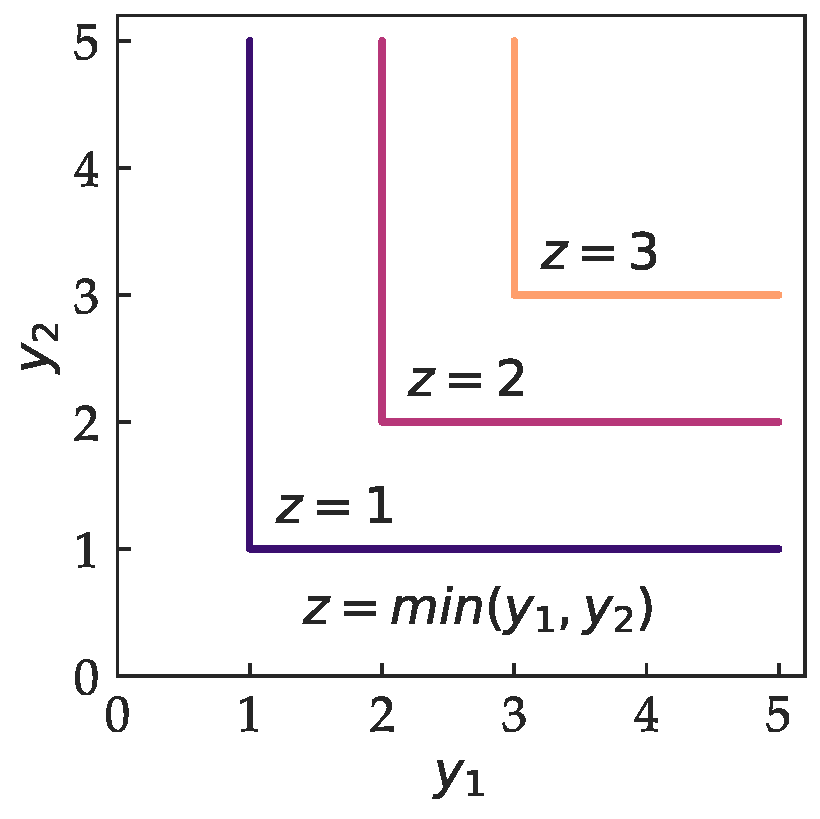
\includegraphics[width=.975\textwidth, height=.975\textwidth]{Figures/Essential.pdf}
    \end{minipage}
    \\ 
    %\begin{minipage}[t]{5cm}
    \uline{Interactive Essential:} Description of the interactive essential relationship.
    %\end{minipage} 
    &
    \begin{minipage}{.175\textwidth}
      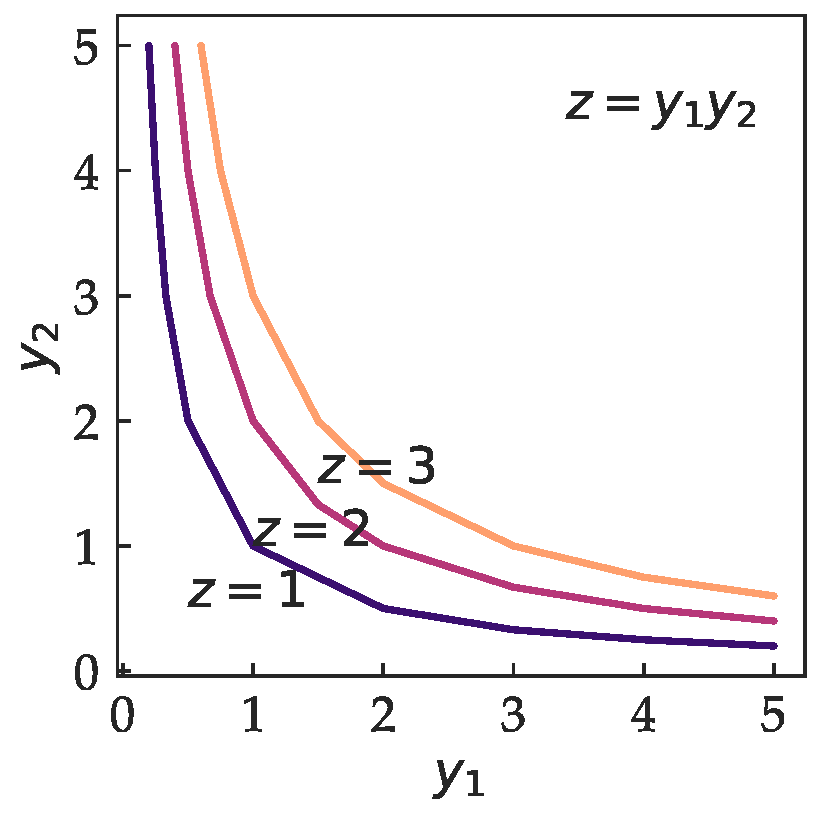
\includegraphics[width=.975\textwidth, height=.975\textwidth]{Figures/Interactive_Essential.pdf}
    \end{minipage}
    \\
    %\begin{minipage}[t]{5cm}
    \uline{Switching:} Description of switching relationship.
    %\end{minipage} 
    &
    \begin{minipage}{.175\textwidth}
      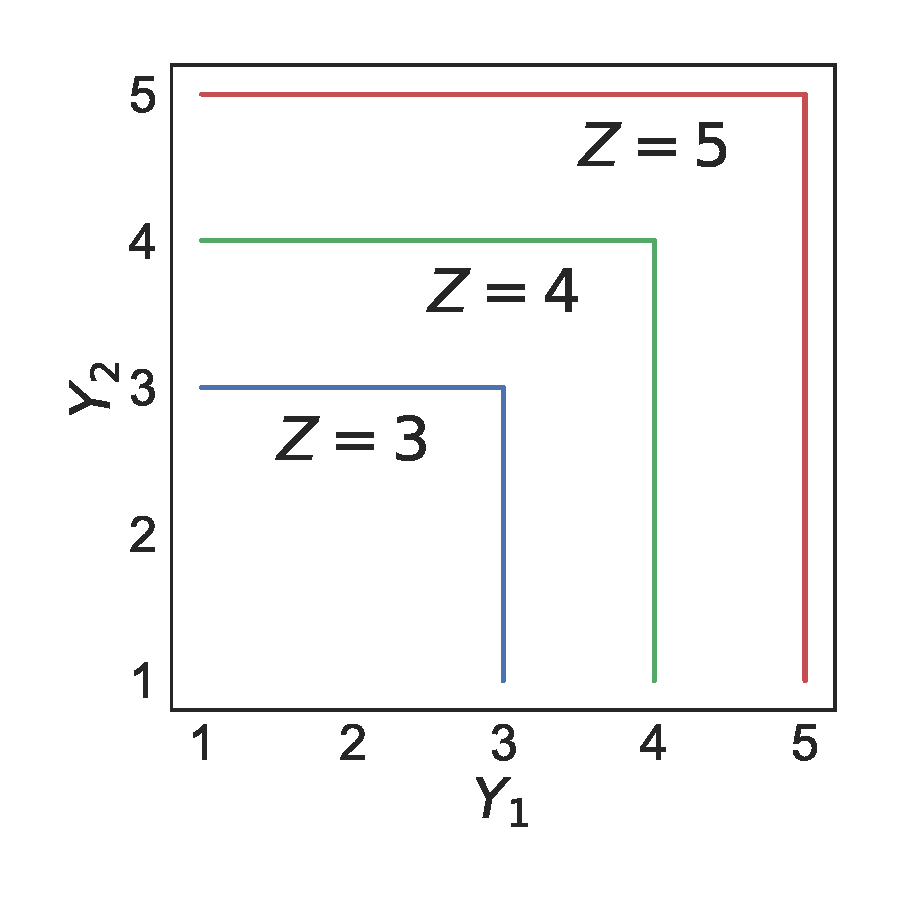
\includegraphics[width=.975\textwidth, height=.975\textwidth]{Figures/Switching.pdf}
    \end{minipage}
    \\
    \hline
  \end{tabular}
  \caption{Pairwise interaction between factors}
  \label{tab:interaction}
\end{table}

\textbf{User to Asker/Answerer/Commenter.} Computing/predicting number of askers/answerers/commenters from number of users. \textcolor{blue}{Figure: Plot to show the correlation between number of users and number of askers/answerers/commenters}



